\documentclass[10pt,a4paper]{report}
\usepackage[utf8]{inputenc}
\usepackage[english]{babel}
\usepackage[T1]{fontenc}
\usepackage{amsmath}
\usepackage{amsfonts}
\usepackage{amssymb}
\usepackage{lmodern}
\usepackage{fancyvrb}
\usepackage{dirtree}
\usepackage{hyperref}		% enabling hyperlinks
\hypersetup{
    colorlinks=true,
    linkcolor=blue, % Couleur des liens internes
    citecolor=red, % Couleur des numéros de la biblio dans le corps
    urlcolor=blue} % Couleur des url
\usepackage{tikz}
\usetikzlibrary{calc}
\usetikzlibrary{arrows}
\usetikzlibrary{shadows}
\usetikzlibrary{patterns}
\usetikzlibrary{positioning}
\usetikzlibrary{shapes}
\usetikzlibrary{3d}
%\usetikzlibrary{automata}
\usetikzlibrary{fit}

\tikzset{block/.style={draw, text centered, fill=gray!10,drop shadow}}
\tikzset{connect/.style={draw, line width=1 pt}}

\tikzset{fifo/.style={draw,rectangle,minimum height=0.2cm,minimum width=0.5cm,preaction={fill=white},pattern=vertical lines,pattern color=black}}

\tikzset{state/.style={block,rectangle,minimum height=1.5cm,minimum width=2cm}}
  
  
  \newcommand{\action}[2]{\path[draw] (#1.east) -- node[draw,rectangle,anchor=west,xshift=0.25cm,text width=6cm]{#2} ++(0.5cm,0);}

\newcommand{\rising}{$\uparrow$}


% ********* head and foot *********
\usepackage{fancyvrb}
\usepackage{etoolbox}
\usepackage{fancyhdr}
%\headheight = 30pt
\pagestyle{fancy}
\fancyhead[LO]{\small\slshape \rightmark}
\fancyhead[RO]{\small\slshape \leftmark}
\renewcommand{\chaptermark}[1]{% 
\markboth{\MakeUppercase{\thechapter.\ }#1}{}}
\renewcommand{\sectionmark}[1]{\markright{\thesection.\ #1}}

\makeatletter
\patchcmd{\@makeschapterhead}{\vspace*{50\p@}}{\vspace*{20\p@}}{}{}
\patchcmd{\DOTIS}{\vskip 40\p@}{\vskip -20\p@}{}{}
\preto{\@verbatim}{\topsep=0pt \partopsep=0pt }
\makeatother

% ********* version *********
\newcommand{\version}{\input{../../version.txt}}

\author{Sebastien CAUX}
\title{GPStudio manual \version}

\begin{document}
\maketitle

%\section*{Developers}

%\newpage

% ========== CONTENTS TABLE ==========
\newpage
\addtocontents{toc}{~\hfill\textbf{Page}\par}
%\setcounter{tocdepth}{1}
\thispagestyle{empty}
\tableofcontents
\thispagestyle{empty}

\chapter*{Introduction}

Smart Cameras allow to embed image processing nearest to image sensors. Embedded systems are therefore deployed to extract high level image features with (pixel-wise) computational intensive operations. Given the limited computational capabilities of embedded devices, programmable FPGA architectures have been proposed to speed-up the processing performance. Such architectures are able to perform high throughput processing within a modular and flexible approach. However, in developing FPGA vision applications one of the biggest issues is the increased development time compared to classical computer vision techniques.

Therefore, with the integration of FPGA devices into smart camera platforms, node programmability becomes a major concern for FPGA developers. In addition of the algorithm transcription using low-level programming languages such as VHDL or Verilog, FPGA designers have also to manage internal circuitry.
%(communication drivers, modules synchronization, interfaces...).
With the time-to-market era, reducing the development time can be a considerable advantage. In this context,
a higher level description would be useful to abstract low-level hardware considerations and increase the added value. 

In this work we propose the \textit{GPStudio} toolchain. It aims at managing low-level hardware abstractions allowing developers to focus on the porting of algorithms into hardware architecture. By leveraging the modular architecture concept, available Intellectual Properties (IP) modules are easily instantiated with standard interfaces between sensors, processing and communication blocks. In this way, a cross-platform IP library is proposed to improve the code re-usability for a wide range of smart camera applications. Once the application is defined, \textit{GPStudio} automatically generates the architecture and the glue code for the targeted board. 
All in all, \textit{GPStudio} allows a rapid FPGA deployment using in-library or custom defined modules (with your preferred HDL language or HLS). With the generated \textit{GPStudio} debug facilities, the FPGA development has never been so easy! 

\chapter{Concepts}

Schema node ex

\section{Blocks}

2 types de blocks

%\subsection{IO}
IO block is an interface between exterior of the node and the inside. It could be a communication with others nodes or sensors. 

%\subsection{Process}
A process block have the capability to transform data witch come from input to processed data depending of internal parameters.

\begin{equation}
fout_{i}=f(\underline{fin}, \underline{parameters})
\end{equation}

It have at least one input and one output, parameters are optional.

\section{Flows}
Flow is a dedicated connexion between a flow interface input and a flow interface output of two blocks. dataflow KPN

\section{Node}
A node in GPStudio is a physical platform, it can be a smart camera or a sensor.

\chapter{Block}
\section{Structure}

\begin{figure}[h!]
\centering
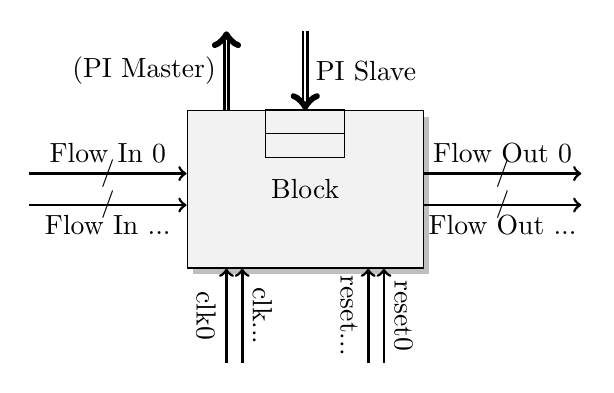
\begin{tikzpicture}
\node[block,rectangle,minimum height=2cm,minimum width=3cm] (bloc) {Block};

\path[connect,<-] ([yshift=0.2cm]bloc.west) -- node{/} node[above]{Flow In 0} ++(-2cm,0);
\path[connect,<-] ([yshift=-0.2cm]bloc.west) -- node{/} node[below]{Flow In ...} ++(-2cm,0);

\path[connect,->] ([yshift=0.2cm]bloc.east) -- node{/} node[above]{Flow Out 0} ++(2cm,0);
\path[connect,->] ([yshift=-0.2cm]bloc.east) -- node{/} node[below]{Flow Out ...} ++(2cm,0);

\path[connect,<-,double] (bloc.north) -- node[right]{PI Slave} ++(0,1cm);
\path[connect,->,double] ([xshift=-1cm]bloc.north) -- node[left]{(PI Master)} ++(0,1cm);

\draw ([xshift=-0.5cm]bloc.north) rectangle ([xshift=0.5cm,yshift=-0.3cm]bloc.north);
\draw ([xshift=-0.5cm,yshift=-0.3cm]bloc.north) rectangle ([xshift=0.5cm,yshift=-0.6cm]bloc.north);

\path[connect,<-] ([xshift=-1cm]bloc.south) -- node[sloped,below]{clk0} ++(0,-1.2cm);
\path[connect,<-] ([xshift=-0.8cm]bloc.south) -- node[sloped,above]{clk...} ++(0,-1.2cm);

\path[connect,<-] ([xshift=1cm]bloc.south) -- node[sloped,above]{reset0} ++(0,-1.2cm);
\path[connect,<-] ([xshift=0.8cm]bloc.south) -- node[sloped,below]{reset...} ++(0,-1.2cm);
\end{tikzpicture}
\caption{Generic block}
\end{figure}

A block is composed of :
\begin{description}
\item[flow interfaces list] with direction and size of data in bits
\item[interface parameter interconnect] configuration of slave and master
\item[internal registers list] with relative address
\item[clocks list] with frequency, domain and shifting phase
\item[resets list] with polarity and reset group
\end{description}

\subsection{flow interfaces}
\subsection{interface parameter interconnect}
\subsection{internal registers list}
\subsection{clocks list}
\subsection{resets list}


\section{Different types of block}
\subsection{Process}
A process is a standard block without any addition data. It have at least one flow input and one flow output. Internal dynamic parameter with slave parameter interface (slave PI) are optional.

\subsection{IO}
An IO is a block with a custom interface externally connected to the node. For example, an image sensor interface is an IO because it have a special connexions to the outside.

\chapter{Flows}
\section{Assumptions}
We assume that the whole design is synchronous to a single clock, clk\_proc.

logic mux

...

\section{Structure}
Flow connexion is composed by three electric signals :
\begin{itemize}
\item a data bus of the size of one data with \emph{\_data} suffix
\item a data valid signal to indicate that a data is present on the data bus with \emph{\_dv} suffix
\item a flow valid signal to delimit the beginning of the flow and the end with \emph{\_fv} suffix
\end{itemize}

\begin{figure}[h!]
\centering
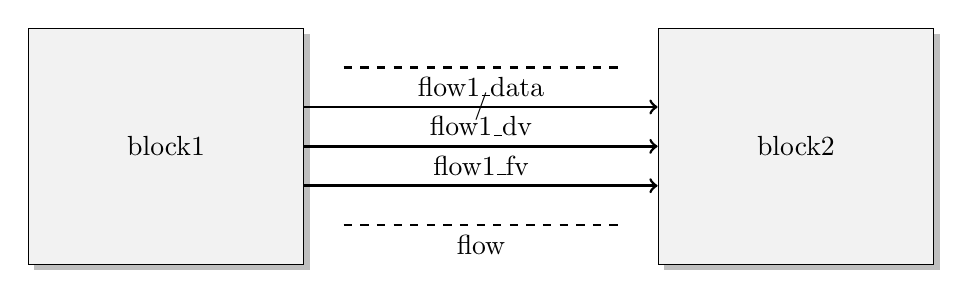
\begin{tikzpicture}[node distance=8cm]
\tikzset{blocstyle/.style={block,rectangle,minimum height=3cm,minimum width=3.5cm}};

% blocks
\node[blocstyle] (bloc1) {block1};
\node[blocstyle,right of=bloc1] (bloc2) {block2};

% Flow to
\path[connect,->] ([yshift=0.5cm]bloc1.east) -- node[above]{flow1\_data} node{/} ([yshift=0.5cm]bloc2.west);
\path[connect,->] (bloc1.east) -- node[above]{flow1\_dv} (bloc2.west);
\path[connect,->] ([yshift=-0.5cm]bloc1.east) -- node[above]{flow1\_fv} ([yshift=-0.5cm]bloc2.west);

% flow tube
\path[connect,dashed] ([xshift=0.5cm,yshift=1cm]bloc1.east) -- ([xshift=-0.5cm,yshift=1cm]bloc2.west);
\path[connect,dashed] ([xshift=0.5cm,yshift=-1cm]bloc1.east) -- node[below]{flow} ([xshift=-0.5cm,yshift=-1cm]bloc2.west);
\end{tikzpicture}
\caption{Details on flow connexion}
\end{figure}

All theses signals are synchronous on clk\_proc clock.

\section{Timing}
\begin{figure}[h!]
\centering
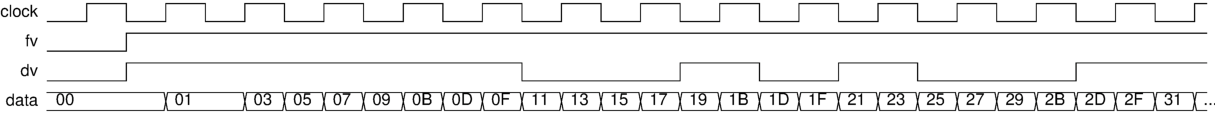
\includegraphics[width=\textwidth]{wave.pdf}
\caption{Example timing for flow signals}
\end{figure}

\section{Clock}
All the flow transmission are synchronous on the same clock, clk\_proc. Like that, we don't need diferent clock domain for data transmission. If a process or IO need to internally work with a different clock, clock syncronisation have to be done internally of the block.
\chapter{Camera Node}
\section{Top level of a node}

\begin{figure}[h!]
\centering
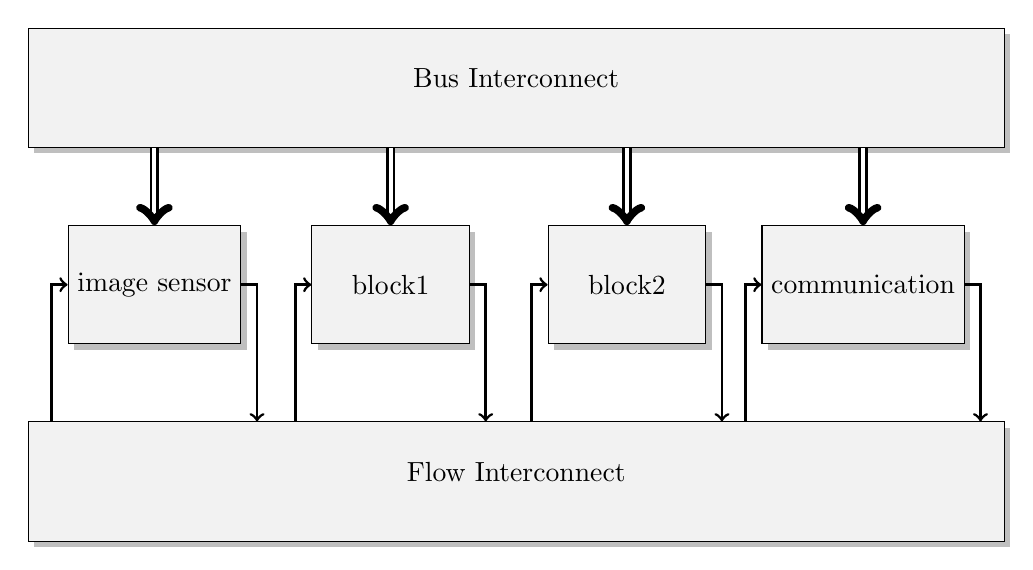
\begin{tikzpicture}[node distance=3cm]
\tikzset{blocstyle/.style={block,rectangle,minimum height=1.5cm,minimum width=2cm}};

% blocks
\node[blocstyle] (bloc1) {image sensor};
\node[blocstyle,right of=bloc1] (bloc2) {block1};
\node[blocstyle,right of=bloc2] (bloc3) {block2};
\node[blocstyle,right of=bloc3] (bloc4) {communication};

% SI
\node[blocstyle,fit=(bloc1) (bloc4),inner xsep=0.5cm,inner ysep=0,yshift=2.5cm] (siwb) {Bus Interconnect};
\node[blocstyle,fit=(bloc1) (bloc4),inner xsep=0.5cm,inner ysep=0,yshift=-2.5cm] (mx) {Flow Interconnect};

% Flow to 
\foreach \s in {1,...,4}
{
    \path[connect,->] (bloc\s.east) -| ([xshift=0.2cm]bloc\s.east |- mx.north);
    \path[connect,<-] (bloc\s.west) -| ([xshift=-0.2cm]bloc\s.west |- mx.north);
    \path[connect,<-,double,double distance=0.5mm] (bloc\s.north) -- (bloc\s.north |- siwb.south);
}
\end{tikzpicture}
\caption{Top level of a node}
\end{figure}

\subsection{Special blocks - Network on chip}

intro noc
is a special block generated by GPS

schema avec FI/PI/CI

\subsubsection{FI - Flow Interconnect}
FI - Flow Interconnect connects and re-assign mapping between flow interface blocks.

All the flow interface of each blocks are connected to FI.

\begin{figure}[h!]
\centering
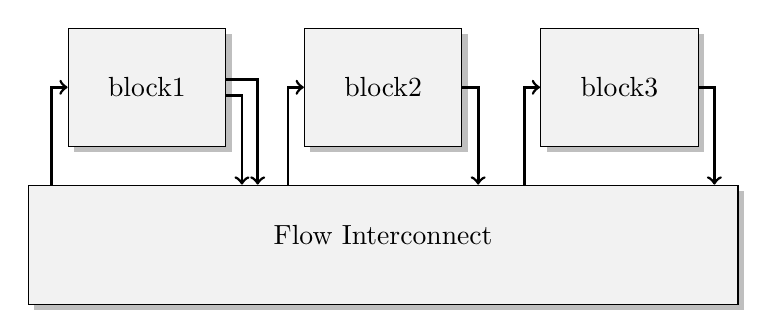
\begin{tikzpicture}[node distance=3cm]
\tikzset{blocstyle/.style={block,rectangle,minimum height=1.5cm,minimum width=2cm}};

% blocks
\node[blocstyle] (bloc1) {block1};
\node[blocstyle,right of=bloc1] (bloc2) {block2};
\node[blocstyle,right of=bloc2] (bloc3) {block3};

% SI
\node[blocstyle,fit=(bloc1) (bloc3),inner xsep=0.5cm,inner ysep=0,yshift=-2cm] (mx) {Flow Interconnect};

% Flow to 
\foreach \s in {2,...,3}
{
    \path[connect,->] (bloc\s.east) -| ([xshift=0.2cm]bloc\s.east |- mx.north);
    \path[connect,<-] (bloc\s.west) -| ([xshift=-0.2cm]bloc\s.west |- mx.north);
}
\path[connect,->] ([yshift=0.1cm]bloc1.east) -| ([xshift=0.4cm]bloc1.east |- mx.north);
\path[connect,->] ([yshift=-0.1cm]bloc1.east) -| ([xshift=0.2cm]bloc1.east |- mx.north);
\path[connect,<-] (bloc1.west) -| ([xshift=-0.2cm]bloc1.west |- mx.north);
\end{tikzpicture}
\caption{FI connexions to blocks}
\end{figure}

This mapping rules are apply :
\begin{itemize}
\item In case of a direct connexion of a flow out interface to one flow input, interface are hard connected through FI.
\item If two flow out are connected to one input, FI create a dynamically configurable multiplexer to permit flow redirection at runtime. This multiplexer is controlled by an internal register.
\end{itemize}

For the size of flow, FI generator process like that :
\begin{itemize}
\item In case of identical size of flow, data of flow interface are connected bit to bit.
\item If the output is larger than the input, an msb connexion is done by default unless you explicitly specify an lsb connexion. Other bits are losted.
\item And if the output is smaller than the input, an msb connexion is done by default unless you explicitly specify an lsb connexion. Zero bits are added as extra bits.
\end{itemize}

ZOOM + explication mux

This block need a special configuration specified in the node project file. This configuration contains all flow connexions between block. It's automatically added by an HDL Toolchain.

\subsubsection{PI - Parameter Interconnect}
PI - Parameter Interconnect is a special block generated by GPS to read/write dynamic parameters of blocks. It connect all masters and slaves BI interface together and create logic control for selecting address space of blocks.

BUS

This block doesn't need any configuration. It's automatically added by an HDL Toolchain.

\subsubsection{CI - Clock Interconnect}
CI or Clock Interconnect is a special block generated by GPS to manage all clocks in the node. It distribute the requested clocks frequency to others blocks taking care of clock domains and clock shifting.

It contains PLL if you need frequency that board can't provide.

This block need a special configuration specified in the node project file. This configuration contains frequency for-each clock domain. It's automatically added by an HDL Toolchain.

%\subsubsection{RI - Reset Interconnect}
%soon available (v0.95)

\section{Properties}
Properties is a way to link block low level hardware registers to high level software controller.

%\input{net.tex}
\chapter{Distribution}

\section{Files organisation}
\begin{figure}[h]
\dirtree{%
.1 GPS distribution root.
   .2 \bfseries bin/.
        .3 gpnode.
        .3 gpviewer.
   .2 \bfseries doc/.
   .2 \bfseries script/.
   .2 \bfseries support/.
        .3 board/.
           .4 board1/.
                .5 board1.dev.
        .3 io/.
        .3 process/.
        .3 toolchain/.
}
\caption{Files tree of the main distribution of GPStudio}
\label{fig:archivetree}
\end{figure}

\section{Files format}
All files used by GPStudio are under XML format with specific extension.

\subsection{.dev}
This file is the definition of a board platform, his capabilities and functionalities.

It contains the toolchain to produce a byte code, special attributes for supporting the board and the list of available peripheral. For each peripheral, 

\subsection{.proc}
files implementation list with type of file and path

\subsection{.io}
Io file definition is quite similar of process file with addition of an external interface.

\subsection{.node}

\section{Tools}
\subsection{gpnode}
gpnode is a command line tool that permit to manage a gptudio node project.

\emph{See also gpnode manual.}

\subsection{gpviewer}
gpviewer is a graphical interface to see results of processing and setting up your smart camera during execution.

\emph{See also gpviewer manual.}

\section{Work flow}


\end{document}
